%!TEX root = ./main.tex

\section[Angle]{Ruler 1: Compare Two Antennas (ArrayTrack)}

% SECTION TIMING: 24:00--42:00 (5 frames). ArrayTrack's story in its own pictures.
% One sentence for the section: the same wavefront reaches each antenna a little
% later, so the phase STEP between neighbours encodes the direction -- and a step is
% a difference, so wrapping is beaten.

% Teaching note (210 s): THE geometry frame; go slowly. Antenna 2 is half a
% wavelength to the right; a wave from angle theta travels an extra (lambda/2) sin
% theta to reach it, i.e. lags by pi sin theta. On the I/Q plane that is the green
% arc between x1 and x2. Invert: theta = arcsin(phase step / pi). Running example:
% 30 degrees -> a quarter turn. Ask why lambda/2: any wider and the step itself wraps.
\begin{frame}{Two antennas hear the wave at two phases}
  \vspace{0.3em}
  \centering
  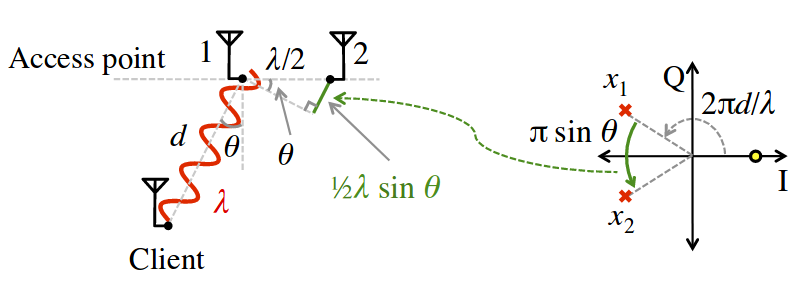
\includegraphics[width=0.88\textwidth]{figure/arraytrack_two_antennas.png}

  \vspace{0.5em}
  \begin{columns}[T,onlytextwidth]
    \column{0.5\textwidth}
      {\small Antenna 2 is $\tfrac{\lambda}{2}\sin\theta$ farther, so it lags by
       $\pi\sin\theta$:\par}
      \vspace{0.2em}
      {\normalsize\centering $\theta = \arcsin\!\big(\tfrac{\angle x_2 -
        \angle x_1}{\pi}\big)$\par}
    \column{0.46\textwidth}
      {\small Phone at $30^\circ$: a \textbf{quarter turn} per antenna.\par}
      \vspace{0.2em}
      {\small Spacing is $\lambda/2$ so the step itself never wraps.\par}
  \end{columns}
  \source{https://www.usenix.org/conference/nsdi13/technical-sessions/presentation/xiong}{Figure: ArrayTrack, NSDI 2013 (as redrawn in Princeton COS463 Lab 5)}
\end{frame}

% Teaching note (180 s): N antennas = N-1 steps; sweep a candidate angle in software
% and ask how well the measured steps fit -- the fit versus angle is the AoA
% spectrum (right). A peak is a bearing; two APs' bearings cross at the client. Say
% "the beam is a for-loop run after reception".
\begin{frame}{More antennas: a spectrum of power vs.\ bearing}
  \vspace{0.2em}
  \begin{columns}[T,onlytextwidth]
    \column{0.47\textwidth}
      \centering
      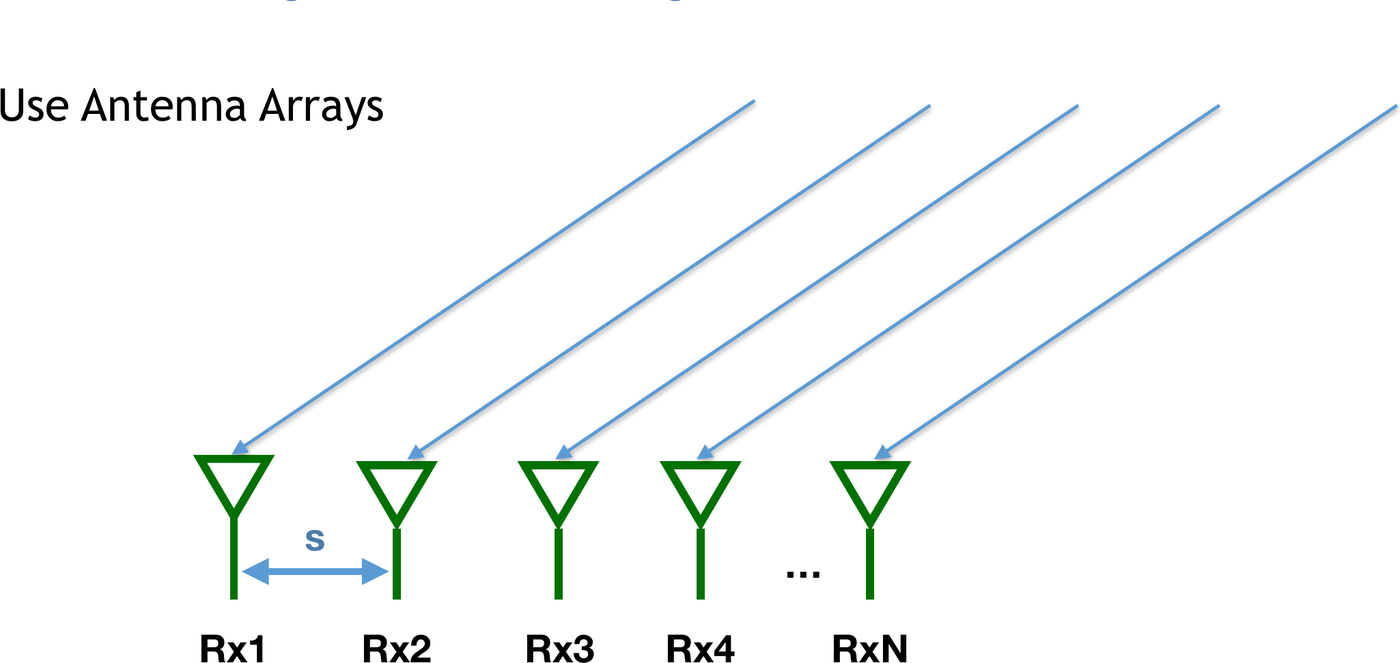
\includegraphics[width=\linewidth]{figure/mit_array.png}
      {\small $N$ antennas, $N-1$ phase steps: sweep $\theta$ in software.\par}
    \column{0.5\textwidth}
      \centering
      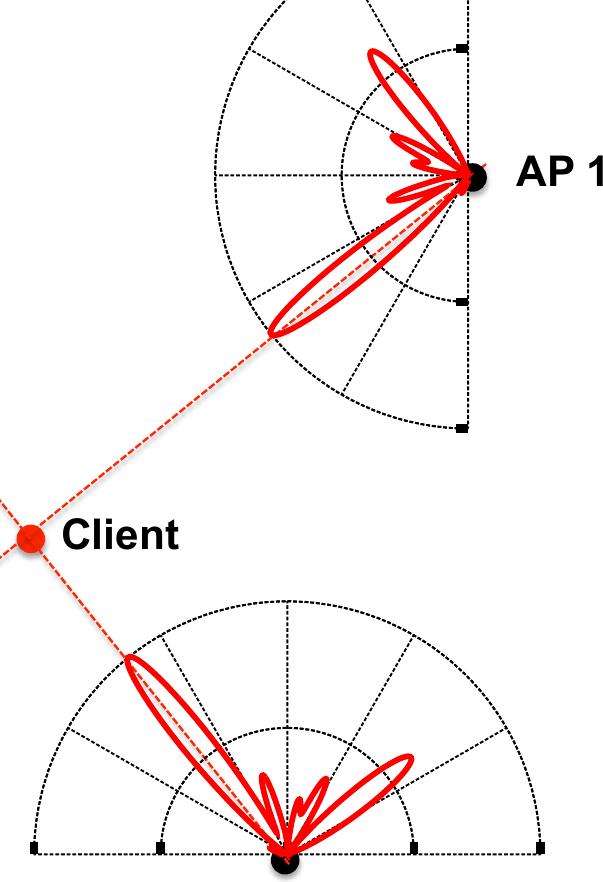
\includegraphics[height=0.52\textheight]{figure/at_approach.png}
  \end{columns}
  \vspace{0.3em}
  \takeaway{A peak in the spectrum is a bearing.\\Two APs' bearings cross at the phone.}
  \source{https://www.usenix.org/conference/nsdi13/technical-sessions/presentation/xiong}{Figures: MIT MAS.S60 Lecture 2 (left); ArrayTrack talk, NSDI 2013 (right)}
\end{frame}

% Teaching note (150 s): reality. Photo: a real office. Diagram: the client's signal
% reaches the array directly (grey), off the wall (green), off furniture (blue) --
% and the spectrum honestly shows ALL of them. Worse: the direct path may be the
% weakest. Leave the question hanging for a beat.
\begin{frame}{The office fights back: multipath}
  \vspace{0.2em}
  \centering
  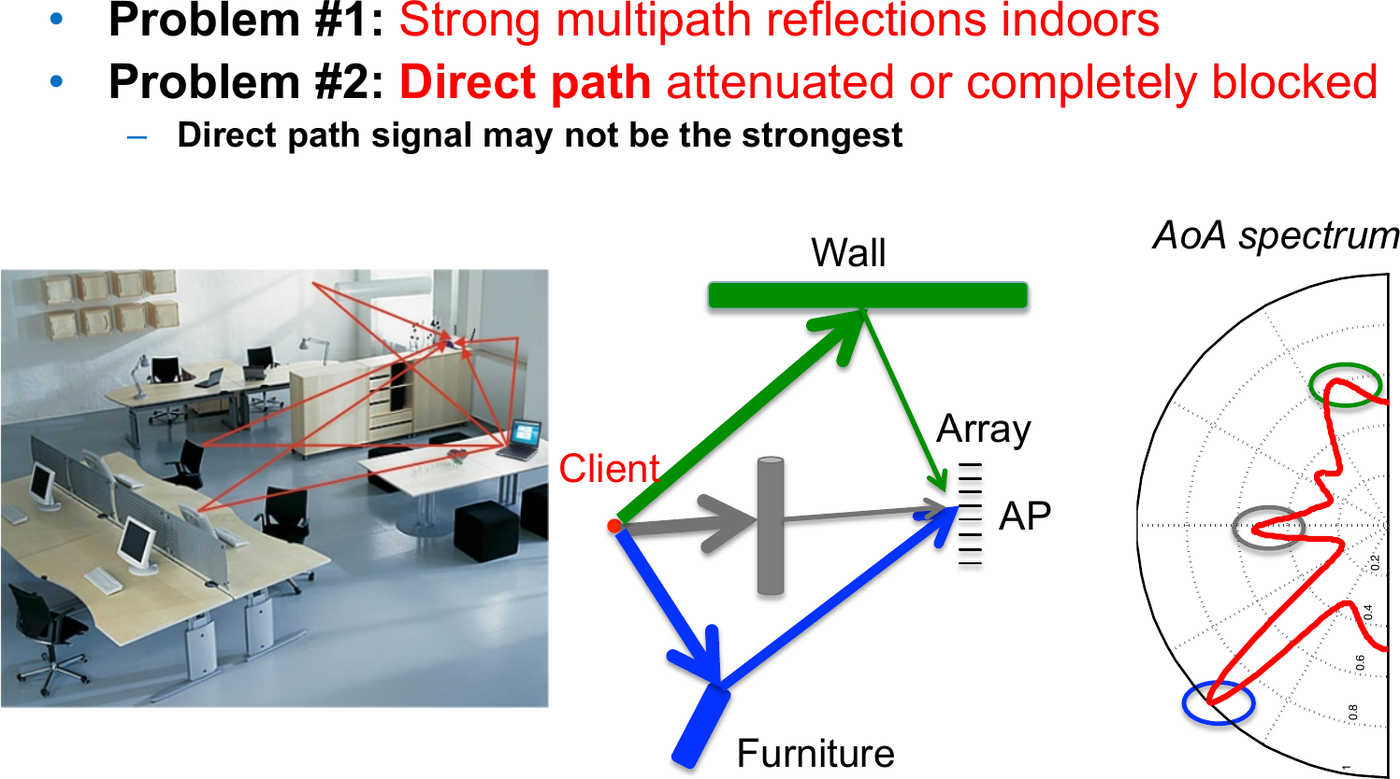
\includegraphics[width=0.9\textwidth]{figure/at_multipath.png}

  \vspace{0.4em}
  \ask{Three lobes in the spectrum. Which one is the phone?}
  \source{https://www.usenix.org/conference/nsdi13/technical-sessions/presentation/xiong}{Figure: ArrayTrack talk, NSDI 2013}
\end{frame}

% Teaching note (180 s): ArrayTrack's answer is physical, not mathematical. Move the
% client a few centimetres: a reflection's bearing swings (the bounce point moves),
% the direct bearing barely changes. Take spectra from two nearby positions and keep
% only peaks that reappear within five degrees.
\begin{frame}{ArrayTrack's trick: the direct path holds still}
  \vspace{0.2em}
  \begin{columns}[T,onlytextwidth]
    \column{0.49\textwidth}
      \centering
      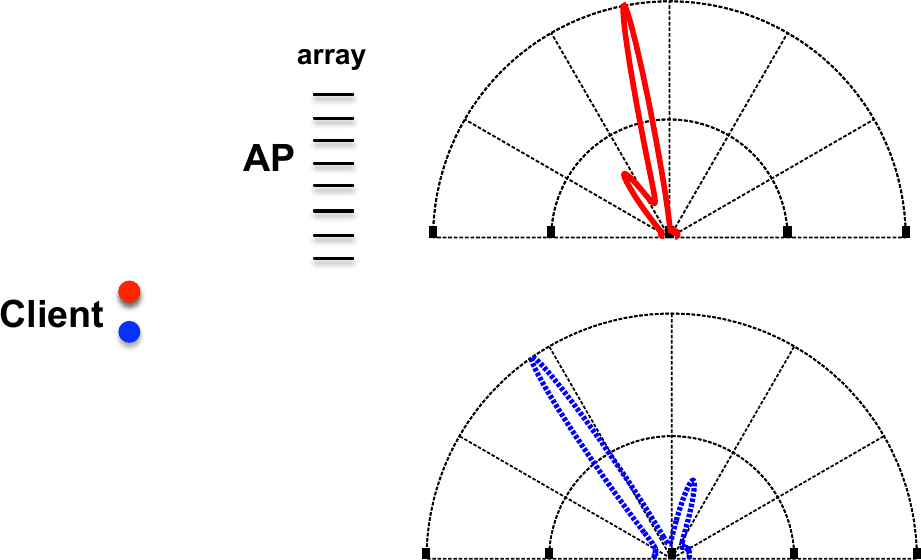
\includegraphics[width=\linewidth]{figure/at_stable_bearing.png}
    \column{0.49\textwidth}
      \centering
      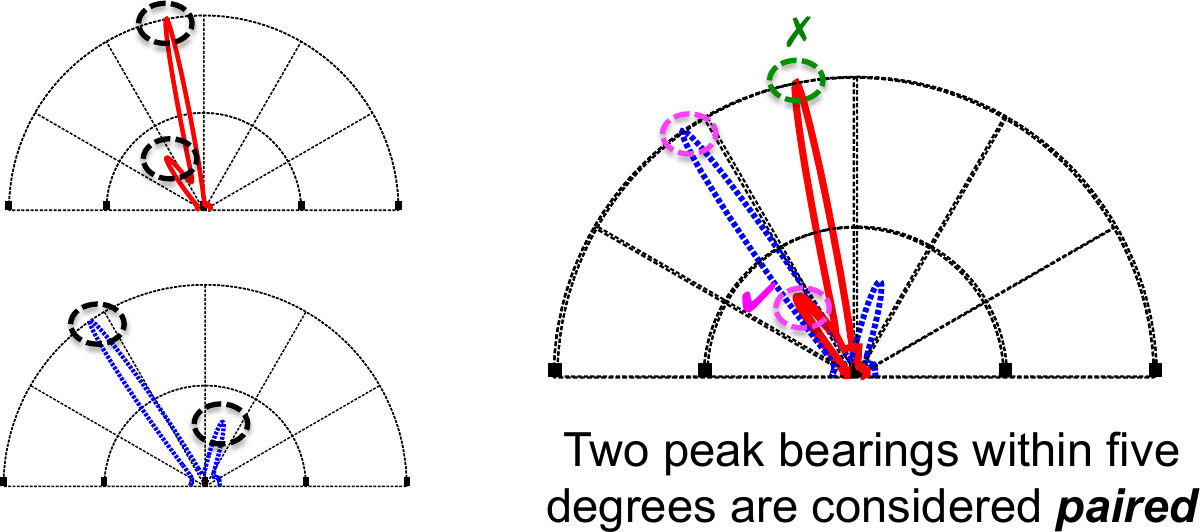
\includegraphics[width=\linewidth]{figure/at_pairing.png}
  \end{columns}
  \vspace{0.4em}
  {\small Move the client a few cm. Reflected bearings swing; the direct bearing
   stays. Keep the peaks that reappear within $5^\circ$.\par}
  \source{https://www.usenix.org/conference/nsdi13/technical-sessions/presentation/xiong}{Figures: ArrayTrack talk, NSDI 2013}
\end{frame}

% Teaching note (150 s): the payoff and the price. One AP gives a bearing, not a
% point; six APs sharpen the heat-map to a dot, 23 cm median. The price is in the
% hardware: six APs, each with 8 antennas, around one room. Last line of the frame
% is the segue -- your home has one AP.
\begin{frame}{More APs, sharper dot: 23 cm}
  \vspace{0.2em}
  \begin{columns}[T,onlytextwidth]
    \column{0.52\textwidth}
      \centering
      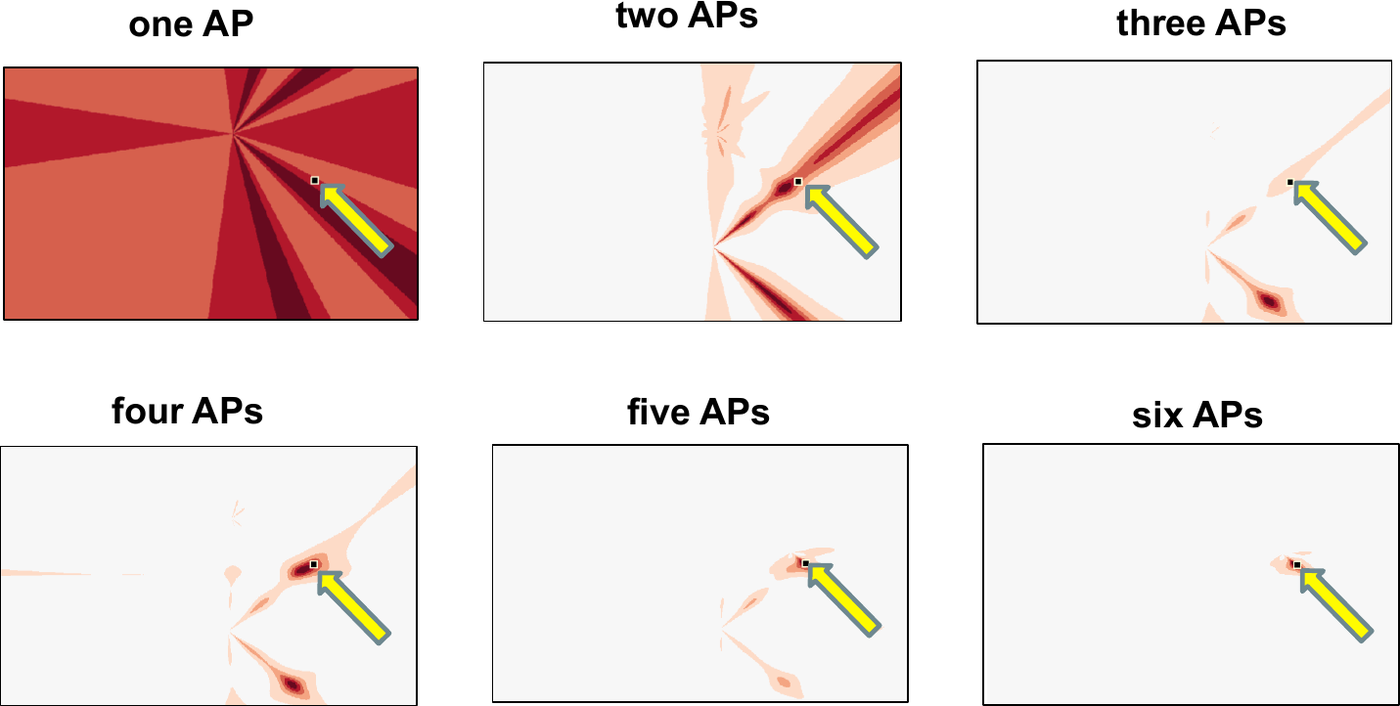
\includegraphics[width=\linewidth]{figure/at_heatmaps_aps.png}
    \column{0.45\textwidth}
      \centering
      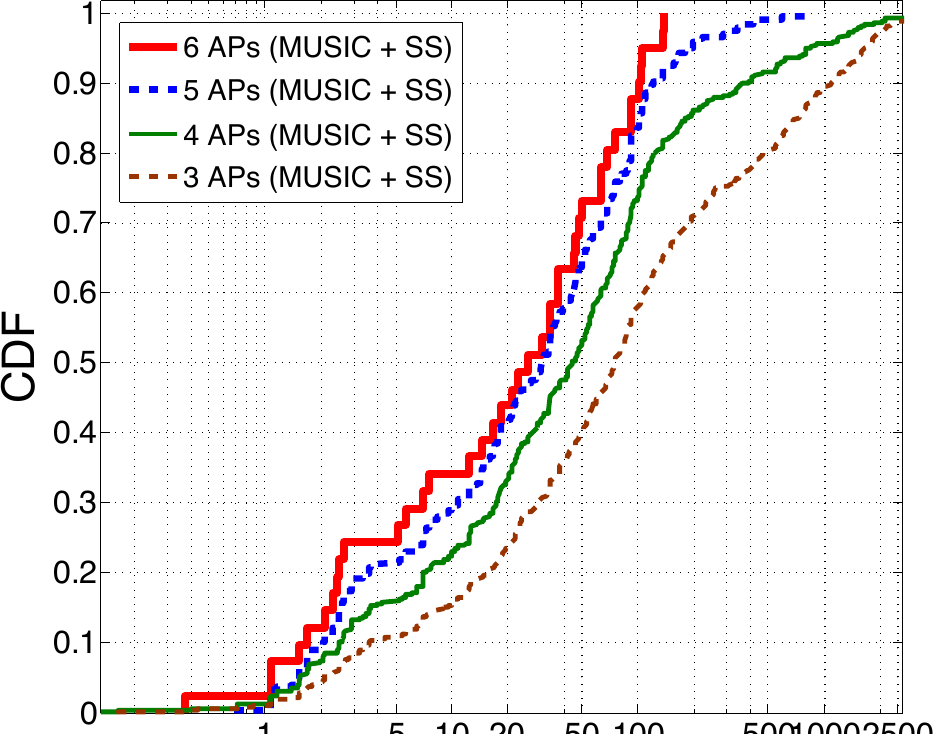
\includegraphics[width=\linewidth]{figure/at_cdf.png}
  \end{columns}
  \vspace{0.3em}
  {\small One AP gives a bearing, not a point. Six 8-antenna APs: \textbf{23 cm
   median}.\par}
  \vspace{0.3em}
  \takeaway{Angle alone needs \emph{several} APs around the room.\\
    Your home has one.}
  \source{https://www.usenix.org/conference/nsdi13/technical-sessions/presentation/xiong}{Figures: ArrayTrack talk, NSDI 2013}
\end{frame}
